\documentclass[12pt]{report}

% Language setting
% Replace `english' with e.g. `spanish' to change the document language
\usepackage[english]{babel}

% Set page size and margins
% Replace `letterpaper' with `a4paper' for UK/EU standard size
\usepackage[letterpaper,margin=1in,marginparwidth=1.75cm]{geometry}

% Useful packages
\usepackage{amsmath,amsthm,amssymb,color,latexsym,mathtools}
\usepackage{graphicx}
\usepackage[]{hyperref}
\usepackage{subfig}
\usepackage{mathtools}
\usepackage{booktabs}
\usepackage{cancel}
\usepackage[all]{xy}
\usepackage{cleveref}
\usepackage{csquotes}

\usepackage[shortlabels]{enumitem}
\usepackage[table]{xcolor}
\usepackage{url}
\geometry{letterpaper}
\usepackage{parskip}


\usepackage[backend=biber]{biblatex}
\addbibresource{citations.bib}

\usepackage[toc]{glossaries}
\loadglsentries{glossary}
\makeglossaries


% \numberwithin{equation}{subsection}

\usepackage{array}
\usepackage{float}
\usepackage[labelfont=bf, font={small,sf}]{caption}
\usepackage{circuitikz}
\usepackage{gensymb}


\setlength{\parindent}{0pt}

\newtheorem{problem}{Problem}

\newtheorem{theorem}{Theorem}
\newtheorem*{proposition}{Proposition}
\newtheorem{lemma}[theorem]{Lemma}
\newtheorem{corollary}[theorem]{Corollary}
\newtheorem{conjecture}[theorem]{Conjecture}
\newtheorem{postulate}[theorem]{Postulate}

\theoremstyle{definition}
\newtheorem{defn}[theorem]{Definition}
\newtheorem{example}[theorem]{Example}

\theoremstyle{remark}
\newtheorem*{remark}{Remark}
\newtheorem*{notation}{Notation}
\newtheorem*{note}{Note}
\usepackage{setspace}

\newenvironment{solution}[1][\it{Solution}]{\textbf{#1. } }{$\square$}

\newcommand{\ndiv}{\not\hspace{2.5pt}\mid}

\setstretch{1}



\begin{document}

\title{robot doggo can learn how to walk???}
\author{Sky Hong}
\date{\today}
\maketitle

\begin{abstract}
    something idk, figure out final formatting later
\end{abstract}

%%%%%%%%%%%%%%%%%%%%%%%%%%%%%%%%%%%%%%%%%%%%%%%%%%%%%%%%%%%%%

\tableofcontents
%\addcontentsline{toc}{chapter}{Glossary}

\chapter{Introduction}

\chapter{Background}
\section{Introduction to Machine Learning}
The field of machine learning is fundamentally about finding functions that model data. For example, a speech recognition model takes audio as an input and outputs a text, and AlphaZero takes a chessboard state as an input and outputs a move. These functions may be vastly complex, with far too many parameters and relations for any human to reasonably articulate and program, even if the task comes naturally to our evolved biology. Machine learning offers methods for computers to achieve these tasks, without the need for a human to give explicit instructions on \textbf{how} it should be accomplished.

This section will give a very introductory overview of machine learning, the specific details of which will be delved more deeply in following sections. The general framework of creating a machine learning model is as follows:

\begin{enumerate}
    \item Identification of the properties of a model. What should this model be able to do? What are its inputs and outputs? What kind of model architecture is best suited to its problem?
    \item Defining a loss function, some metric to measure how well a model performs.
    \item Optimizing the parameters of a model to minimize the loss function and maximize performance.
\end{enumerate}

\subsection{Parameters}

As an example, consider a simple model consisting of a linear relationship between inputs and outputs.
\begin{equation}
    f(\mathbf{x}) = b +\sum_i w_i x_i
\end{equation}

Parameters that directly multiply values, $w_i$, are called \textbf{\glspl{weight}}, and parameters that offset values, $b$, are called \textbf{\glspl{bias}}. This can be generalized to vector outputs as
\begin{equation}
    f = \mathbf{b} + W\mathbf{x} ,
\end{equation}
where $W$ is now a matrix.

The parameters of a model are usually collectively referred to as a vector $\theta$, with components of the individual weights and biases of the model. For complex models, $\theta$ may be millions, billions, or even trillions of parameters long, populated by numerous parameter tensors.
\begin{equation}
    \mathbf{\theta} = \begin{bmatrix}
        W_{11} \\
        W_{12} \\
        \vdots \\
        b_1 \\
        b_2 \\
        \vdots
    \end{bmatrix}
\end{equation}
For virtually all non-trivial problems, linear relationships are far too reductive to completely capture the complexity of a problem. Such inherent limitations of a model due to its architecture known as \textbf{\gls{model-bias}}. Model architectures will be expounded upon in more detail in Section 1.2.

\subsection{Loss Functions}

A \textbf{\gls{loss-function}} (also sometimes called a \textbf{cost function}), typically denoted $L(\theta)$ or just $L$, is the measure of how ``bad'' a set of parameters $\theta$ for a model is. A common definition is the deviation between a model's prediction and an actual result. For example, when building a speech recognition model, the loss may be defined as the error rate between its output transcription and the correct transcription. The training data that is provided to the model, in this case, the correct transcriptions, are identified with \textbf{\glspl{label}} that tell the model what it should train towards.

Losses over all labels in the training data are aggregated into an value for the overall loss function, the most common method of which is the \textbf{\gls{mse}}:
\begin{equation}
    L = \frac{1}{N}\sum (y - \hat{y})^2 .
\end{equation}

$L$ is associated with an \textbf{\gls{error-surface}} that can be understood as the plot of $L$ in a $|\mathbf{\theta}|$-dimensional parameter space, though it is usually far too complex to be directly visualized.

\subsection{Optimization}

Since $L$ is continuous, there must exist some set of parameters $\mathbf{\theta}^\ast$ that minimize $L$ and model the training data best.
\begin{equation}
    \mathbf{\theta}^\ast = \arg\min_{\mathbf{\theta}} L
\end{equation}
The process of improving the model by finding values for $\mathbf{\theta}$ that lower the loss function is what it really means for a model to ``learn'' or ``train''.

\subsubsection{Gradient descent}

Since brute-forcing the error surface of $L$ is infeasible with a large number of parameters, the standard algorithmic approach to find minima of $L$ is \textbf{gradient descent}. In gradient descent, $L$ is iteratively lowered by stepping $\theta$ against the gradient of $L$.
\begin{equation}
    \mathbf{\theta}_{n+1} = \mathbf{\theta}_n-\eta\nabla L(\mathbf{\theta}_n)
\end{equation}
The \textbf{learning rate}, $\eta$, determines the scaling for the size of each step.

\begin{figure}[h]
    \centering
    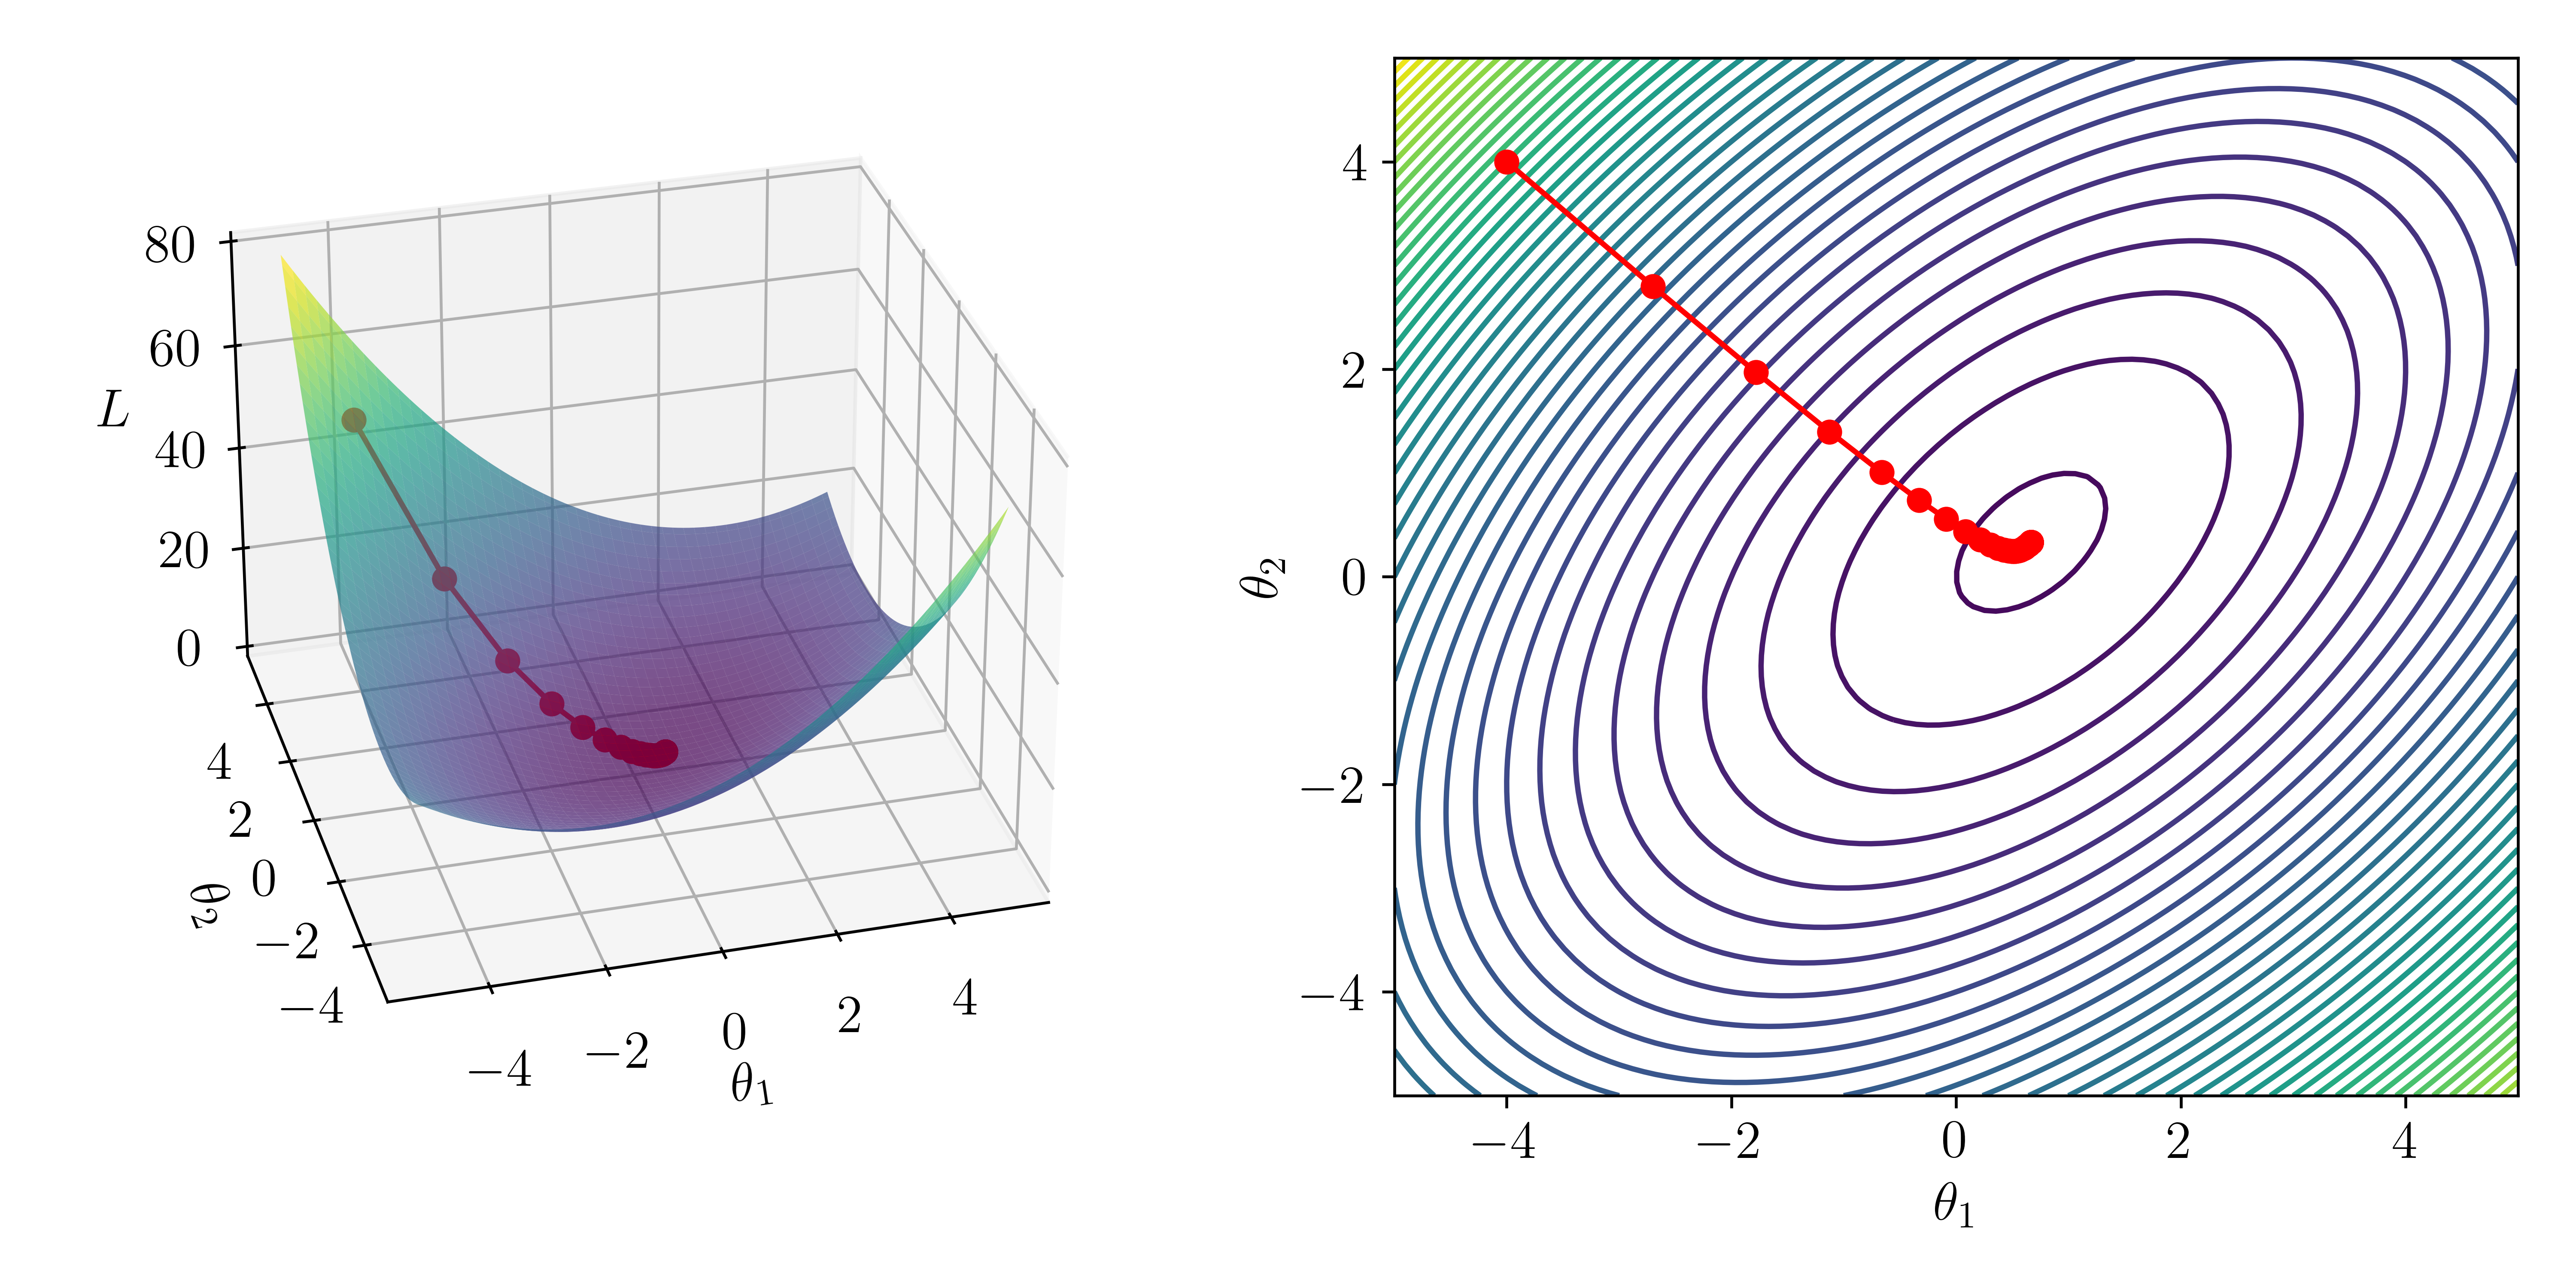
\includegraphics[width=0.7\linewidth]{figs/gradient_descent.png}
    \caption{Visualization of gradient descent on an error surface with two parameters. Darker color indicates smaller $L$. From the Cornell University Computational Optimization Open Textbook, will replace with better figure.}
    \label{fig:enter-label}
\end{figure}

In practice, some conditions may be defined to determine when to cease training, such as setting an upper limit on the number of iterations, setting a time limit, or setting a threshold for a satisfactory value of $L$. These values that modify aspects of a model's learning are called \textbf{\glspl{hyperparameter}}. Hyperparameter optimization is itself a complex topic that is beyond the scope of this section.

When $\mathbf{\theta}$ reaches a critical point ($\nabla L = 0$), the updates to $\mathbf{\theta}$ vanish, and the algorithm has reached a stable ending point. In an ideal case, this would be the global minima of $L$, the best that the model could possibly reach given the training data. In reality, reaching the global minima is highly improbable, $\mathbf{\theta}$ is much more likely to be stuck at a local minima, or a saddle point. We will discuss methods to overcome these challenges in following sections.

\section{Neural Networks}

\textbf{Artificial neural networks (ANNs)}, often shortened to \textbf{Neural Networks (NNs)}, are one of the largest classes of models used in machine learning.

\subsubsection{Activation functions}

For virtually all non-trivial problems, a linear relationships are far too reductive to completely capture the complexity of the task at hand. To model more complex relationships, a variety of non-linear \textbf{activation functions} can process the inputs.

\textbf{Sigmoid functions} are ubiquitous in this role, though other classes of activation functions will also be mentioned later.
\begin{equation}
    \sigma(x) = \frac{1}{1+e^{-x}}
\end{equation}
\begin{figure}[h]
    \centering
    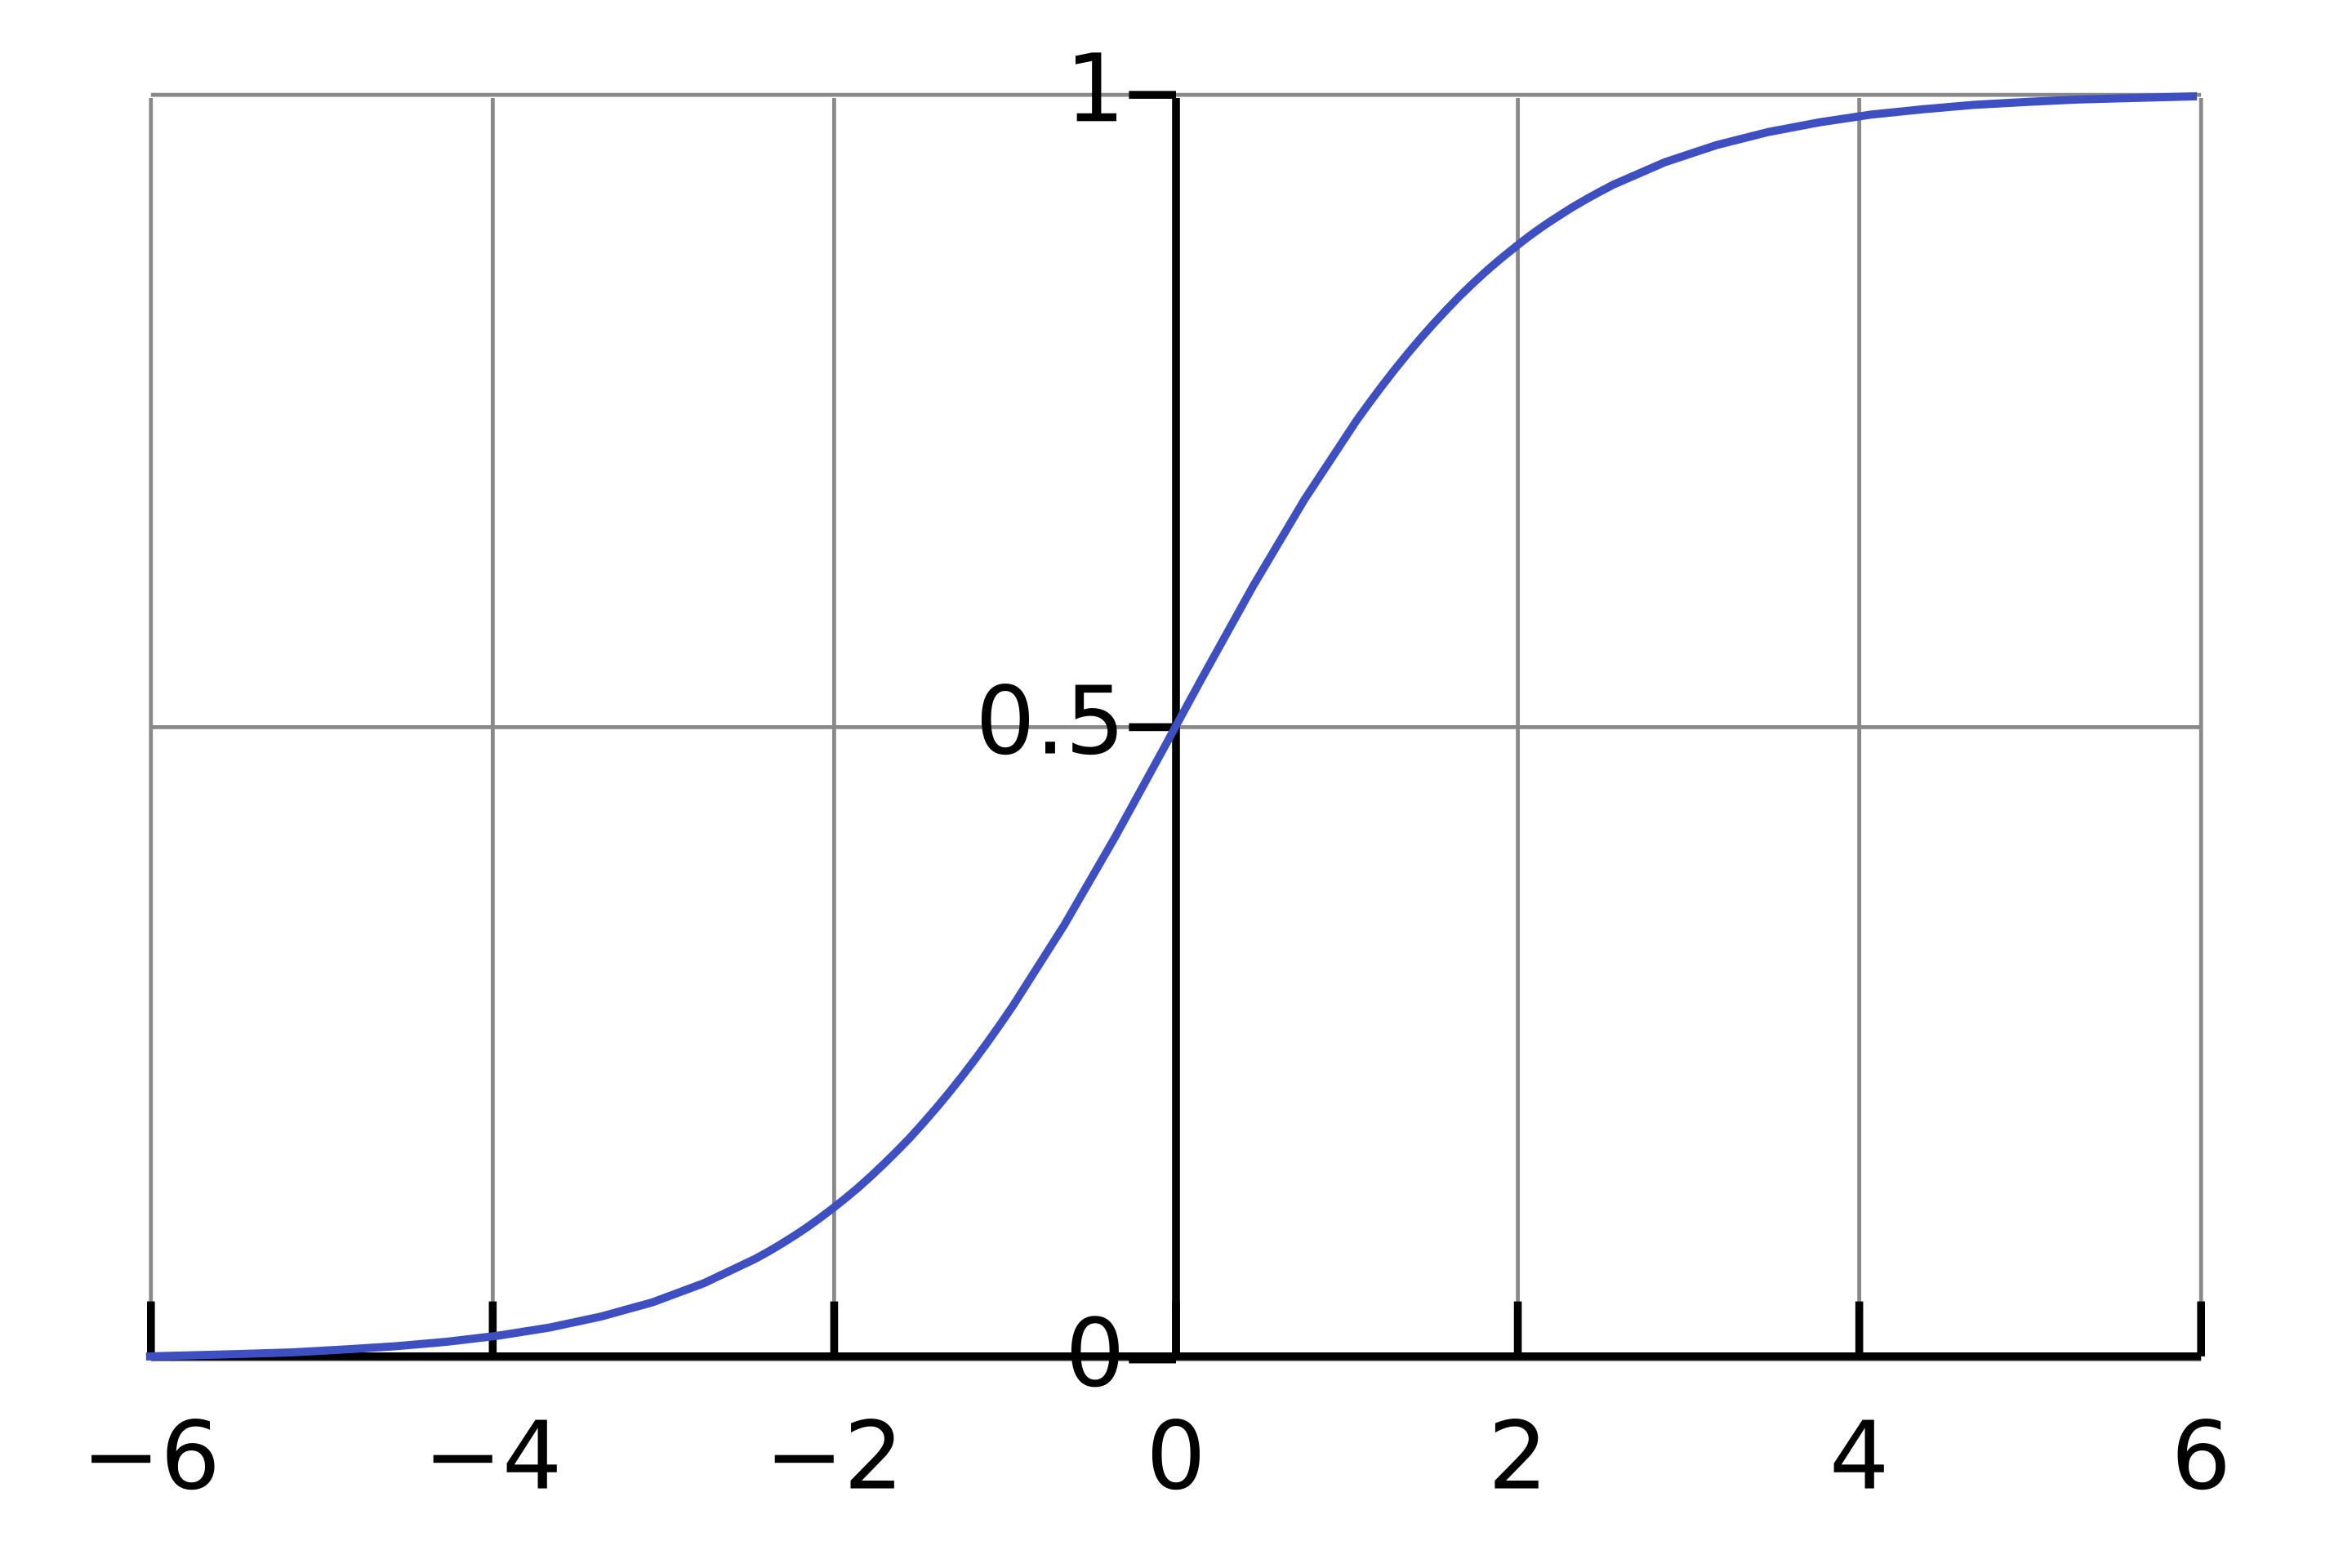
\includegraphics[width=0.5\linewidth]{figs/image.png}
    \caption{replace this with own figure}
    \label{fig:enter-label}
\end{figure}

Any continuous relationship between two variables can be approximated by a sufficiently large linear combination of sigmoid functions. (Note that we define $\sigma$ to act component wise on vector inputs.)
\begin{equation}
    f \approx b + \mathbf{w} \cdot \sigma(\mathbf{b} + W\mathbf{x}).
\end{equation}
This property is formalized more rigorously in the \textbf{Universal Approximation Theorem}.\cite{hornik1989multilayer}

Sigmoid functions also have the advantage that


\section{Backpropagation}

\textbf{Backpropagation} is the textbook algorithm for computing the gradient of the loss function, as in practice, the error surface is almost never computable.



\section{Overfitting}

\section{Variations on Gradient Descent}

\section{Reinforcement Learning}

\chapter{Robotic Systems}

\section{ANYmal by ANYbotics}

\chapter{Literature}

\printglossaries

\printbibliography
\addcontentsline{toc}{chapter}{Bibliography}

\end{document}